% mainfile: ../Refinement.tex
\begin{figure}[h]
\centering
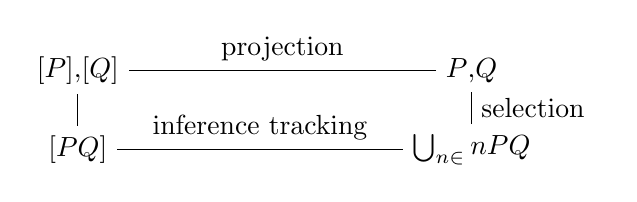
\begin{tikzpicture}
	\node   			(A)	{$\traces[P]$,$\traces[Q]$};
	\node[right of=A, xshift=40mm]	(B)	{$\trI{P}$,$\trI{Q}$};
	\node[below of=B]		(C)	{$\bigcup_{n\in\N}\tracesI{n}{P}{Q}$};
	\node[below of=A]		(D)	{$\traces[\procpar{P}{Q}]$};
	\path	(B)    edge node[anchor=south]  {projection}            (A)
		(C)    edge node[anchor=west, text width=15mm]   {selection}    (B)
		(D)    edge node[anchor=south]  {inference tracking}		(C);
	\path   (D)    edge[draw,decorate,decoration={snake, post=lineto, post length=4mm}] 
			    node[anchor=east]   {} (A);
\end{tikzpicture}
\caption{Visualization of the compositionality of the parallel operator (Part II).}
\label{fig_exp_comp_para2}
\end{figure}
